\documentclass[11pt, letterpaper, includehead]{article}

%%%%%%%%%%%%%%%%%%%%% Pre-document %%%%%%%%%%%%%%%%%%%%%
\usepackage{fancyhdr}  % Allow for headers
\usepackage{graphicx}  % Allow for figures 
\usepackage{float}     % Allow for figure inserted in specified location
\usepackage{xcolor}

\setlength{\parindent}{0pt} % Remove auto paragraph indents

% Get rid of those big ass margins
\usepackage[margin=1in]{geometry}

\begin{document}
  %%%%%%%%%%%%%%%%%%%%% Title Page %%%%%%%%%%%%%%%%%%%%%
  \begin{titlepage} 
    \begin{center}
      \Huge{\textbf{Lab 1}}\\
      \Huge{Motion diagrams}
      \vfill
      \large{\textbf{Rectangle Repulsed Researchers}}\\
      \large{Julian Barossi, Liam Gilligan, Stephanie L'Heureux}\\
      \vspace{0.5cm}
      \normalsize
      \today
    \end{center}
  \end{titlepage}

  %%%%%%%%%%%%%%%%%%%%% TABLE OF CONTENTS %%%%%%%%%%%%%%%%%%%%%
  \tableofcontents
  \pagebreak % Move to next page


  % Add a nice fancy header
  \pagestyle{fancy}
  \fancyhead{}
  \fancyhead[C]{\textbf{Lab 1:} Motion diagrams}

  
  \setcounter{section}{2} % Make numbers start at 3
  \section{Matching Position vs. Time and Velocity vs. Time Graphs}

  %%%%%%%%%%%%%%%%%%%%% GRAPH 2 %%%%%%%%%%%%%%%%%%%%%
  \subsection{Graph 1}

  \begin{figure}[H] % H makes the figure insert at the position in the document
    \centering 
    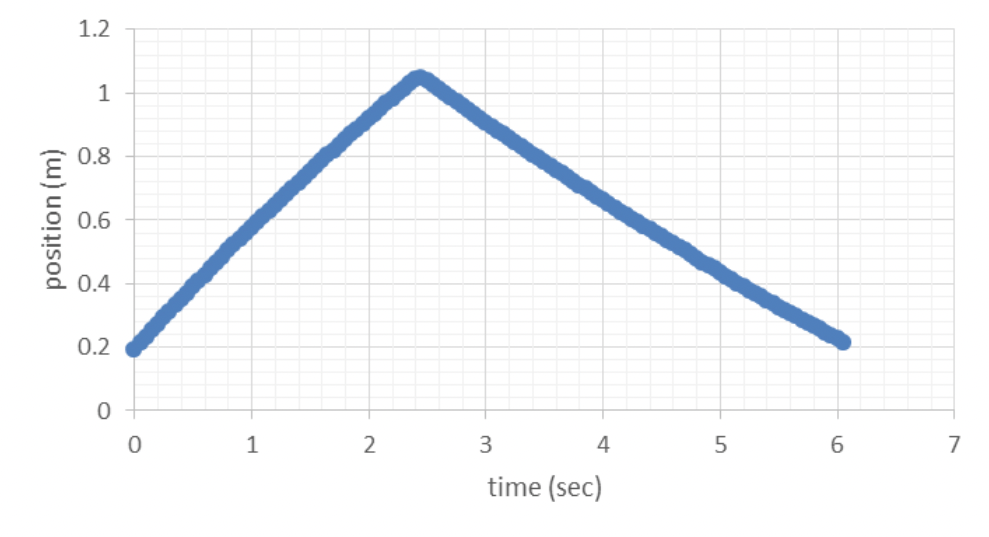
\includegraphics[width=\linewidth]{graph_1.png}
  \end{figure}

  \subsubsection{Graph analysis}
  \emph{Graph 1} describes the position vs. time graph of a collision.
  The graph directly conveys that initially the object's position from the sensor increases, then at
  $t\approx2.4s$ it's position begins decreasing. The derivative of a position vs. time graph gives the velocity. 
  From the slope of the graph, one can conclude that the velocity over the interval $t\epsilon[0s, 2.4s)$
  is constant and positive. Then from $t \epsilon (2.4s, 6s]$ the velocity becomes negative. With this 
  information, one can deduce the object of interest was given an initial velocity and began moving
  in the positive direction, then it encountered a barricade and reversed direction.
  $$\forall \, t \in [0s, 2.4s); \, v(t) = \frac{d}{dt}[s(t)] \approx \frac{0.95m - 0.6m}{2s - 1s} = 0.35 \, m/s$$
  $$\forall \, t \in (2.4s, 6s]; \, v(t) = \frac{d}{dt}[s(t)] \approx \frac{0.95m - 0.7m}{3s - 4s} = -0.25 \, m/s$$

  \subsubsection{Setup}
  The equipment used to recreate \emph{Graph 1} consisted of a level track with a magnetic 
  bumper mounted $60cm$ from the \emph{PASCO Motion Sensor II}. Our lab group pushed and released the cart 
  towards the bumper. The \emph{PASCO Universal 850 Interface} was used to track the motion with sonar. We consider 
  friction and drag negligible in this application.\\

  %%%%%%%%%%%%%%%%%%%%% GRAPH 2 %%%%%%%%%%%%%%%%%%%%%
  \subsection{Graph 2}

  % Centered figure in text location
  \begin{figure}[H] % H makes the figure insert at the position in the document
    \centering 
    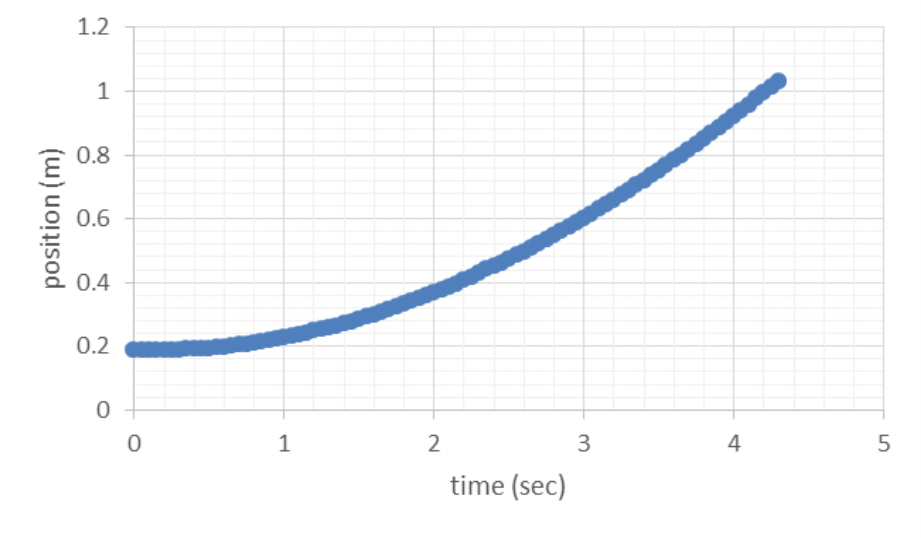
\includegraphics[width=\linewidth]{graph_2.png}
  \end{figure}

  \subsubsection{Graph analysis}
  \emph{Graph 2} depicts an object whose speed is increasing at a constant rate. This deduction is 
  justified by graphical analysis. The position increases over the interval 
  $t\epsilon[0s, 4.3s)$ at a constant rate, resembling a parabolic curve. The derivative of the 
  position vs. time graph yields velocity, which for this plot is increasing and positive. One 
  possible senerio that would recreate the graph is an object which accelerates down an inclined plane.\\
  
  \subsubsection{Setup}
  Our setup consisted of a track angled at an downward incline. We released the cart from the 
  top of the track and let it slide to the bottom towards the \emph{PASCO Motion Sensor II}. The 
  \emph{PASCO Universal 850 Interface} was used to plot motion data collected with sonar. We consider 
  friction and drag negligible in this application.\\
  
  %%%%%%%%%%%%%%%%%%%%% GRAPH 3 %%%%%%%%%%%%%%%%%%%%%
  \subsection{Graph 3}

  \begin{figure}[H] % H makes the figure insert at the position in the document
    \centering 
    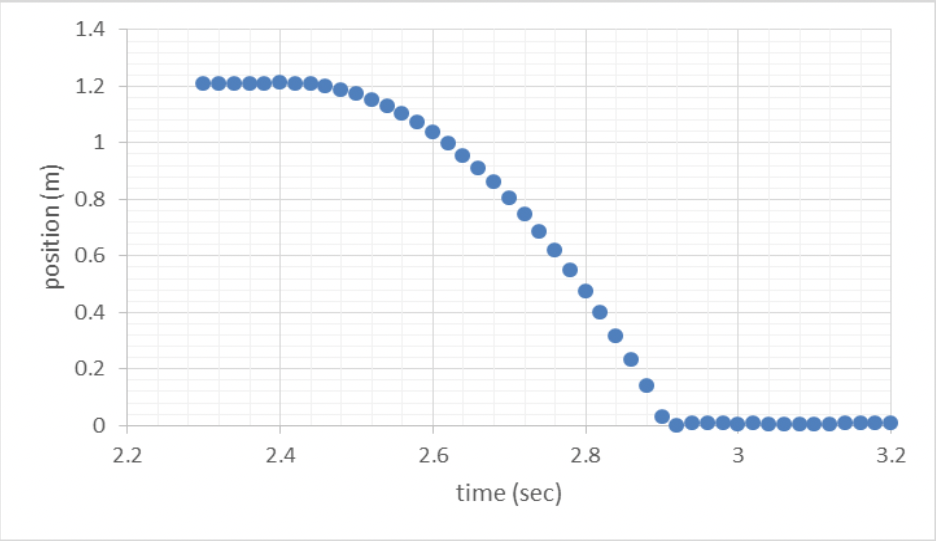
\includegraphics[width=\linewidth]{graph_3.png}
  \end{figure}

  \subsubsection{Graph analysis}
  Graph three depicts an object in freefall that hits the ground and stays there. We know this because the
  object's position starts from an increased height\\
  
  \subsubsection{Setup}
  Our setup consisted of a the sensor positioned updward. We dropped a large beach ball.\\

  %%%%%%%%%%%%%%%%%%%%% GRAPH 4 %%%%%%%%%%%%%%%%%%%%%
  \subsection{Graph 4}

  \begin{figure}[H] % H makes the figure insert at the position in the document
    \centering 
    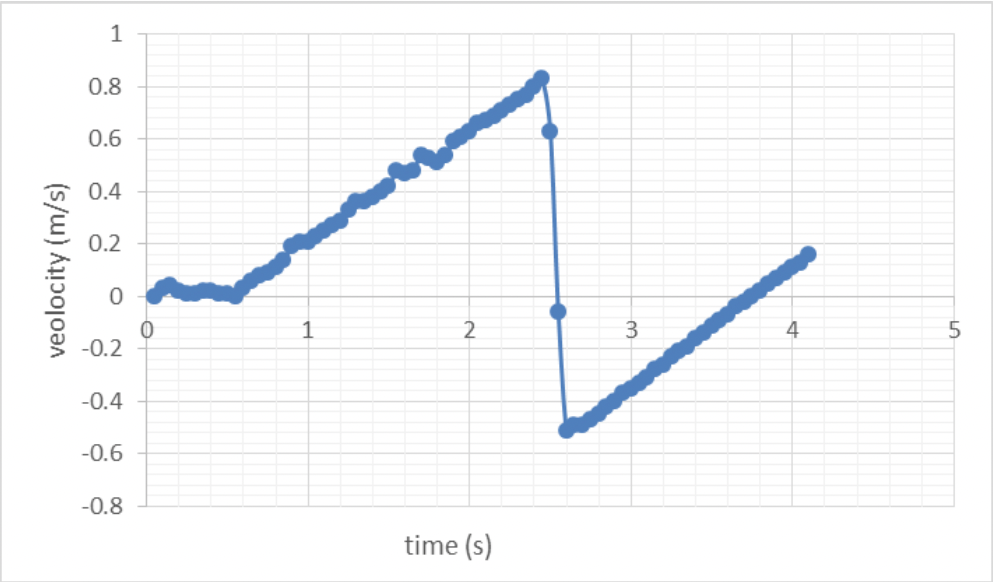
\includegraphics[width=\linewidth]{graph_4.png}
  \end{figure}

  \subsubsection{Graph analysis}
  \emph{Graph 4} depicts an object moving down an incline. It comes in contact with somethinhg at the
  bottom and changes direction. As it changes direction it slows down. Then at $t=2.6s$ its velocity 
  becomes negaiive but the acceleration staus positive where it is slowing down\\
  $$\forall \, t \in [0s, 2.6s); \, a(t) = \frac{d}{dt}[v(t)] \approx \frac{0.6 \, m/s - 0.2 \, m/s}{2s - 1s} = 0.4 \, m/s^2$$
  $$\forall \, t \in (2.6s, 4.1s]; \, a(t) = \frac{d}{dt}[v(t)] \approx \frac{-0.5 \, m/s -(-0.4 \, m/s)}{2.6s - 2.8s} = 0.3 \, m/s^2$$ % Should be 0.4
  
  \subsubsection{Setup}
  Our setup consisted of a the sensor positioned at the biotton of an incline plane. We released the cart from the top 

  %%%%%%%%%%%%%%%%%%%%% GRAPH 5 %%%%%%%%%%%%%%%%%%%%%
  \subsection{Graph 5}

  \begin{figure}[H] % H makes the figure insert at the position in the document
    \centering 
    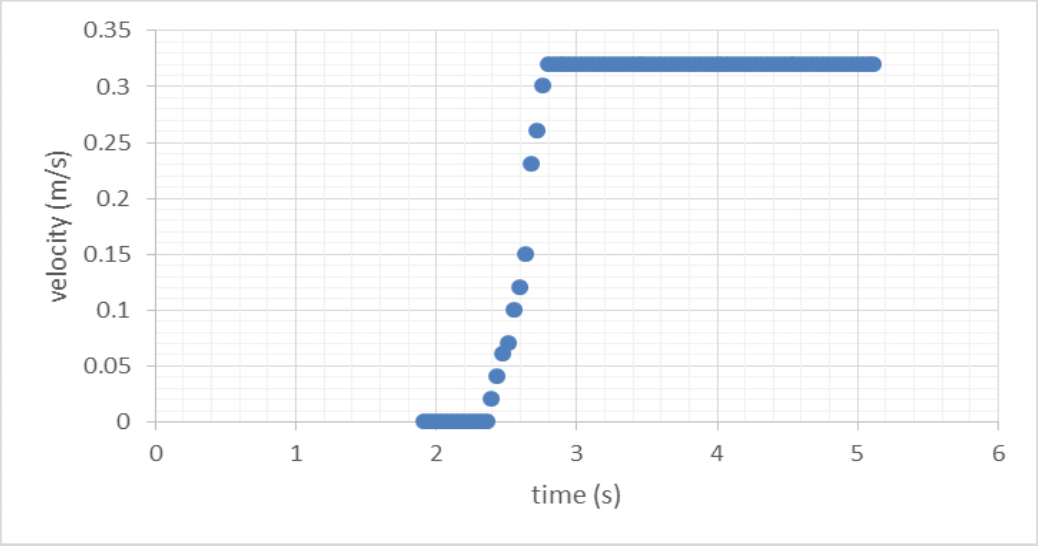
\includegraphics[width=\linewidth]{graph_5.png}
  \end{figure}

  \subsubsection{Graph Analysis}
  Graph 5 depicts an object that starts from rest then is that ts pushed then slows to a stop. 
  We know this because the graph depicts the initial velocity as $0m/s$, then the velocity rapidly 
  increases and the acceleration is posiyive. It the acceleratyion goes to zero and he velocity is constant
  $$\forall \, t \in (2.4s, 2.8s); \, a(t) = \frac{d}{dt}[v(t)] \approx \frac{0.1 \, m/s - 0.24 \, m/s}{2.6s - 2.7s} = 1.4 \, m/s^2$$


  \subsubsection{Setup}
  Our setup consisted a flat plane and pushed the cart away from the sensor


  %%%%%%%%%%%%%%%%%%%%% GRAPH 6 %%%%%%%%%%%%%%%%%%%%%
  \subsection{Graph 6}

  \begin{figure}[H] % H makes the figure insert at the position in the document
    \centering 
    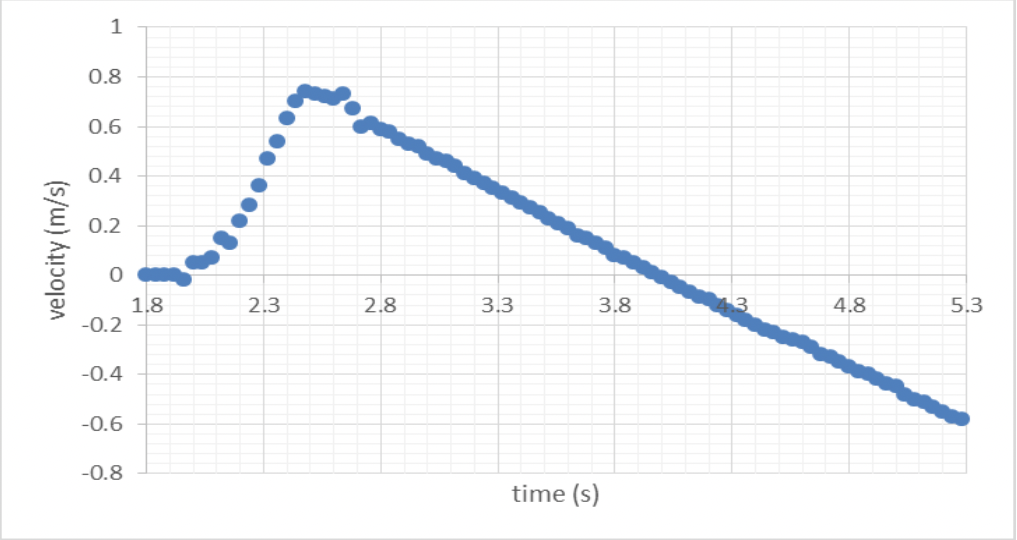
\includegraphics[width=\linewidth]{graph_6.png}
  \end{figure}

  \subsubsection{Graph Analysis}
  The graph above depicts an object being sped up rapidly before decelerating
  at a constant rate.
  $$\forall \, t \in (2, 2.5s); \, a(t) = \frac{d}{dt}[v(t)] \approx \frac{0.08 \, m/s - 0.38 \, m/s}{2.1s - 2.3s} = 1.5 \, m/s^2$$
  $$\forall \, t \in (2.6s, 4.1s]; \, a(t) = \frac{d}{dt}[v(t)] \approx \frac{0.6 \, m/s -(-0.4 \, m/s)}{2.8s - 4.8s} = -0.5 \, m/s^2$$ 
  % Graph 6: ~ −0.53m/s/s
  \subsubsection{Setup}
  To recreate the motion described by the graph, we decided to use an inclined plane.
  The graph initially shows a positive acceleration, but later a constant negative acceleration.
  To recreate this on the inclined plane, we pushed the cart up, then let
  gravity slow it down and accelerate it back down the incline.

  %%%%%%%%%%%%%%%%%%%%% GRAPH 7 %%%%%%%%%%%%%%%%%%%%%

  \subsection{Graph 7}

  \begin{figure}[H] % H makes the figure insert at the position in the document
    \centering 
    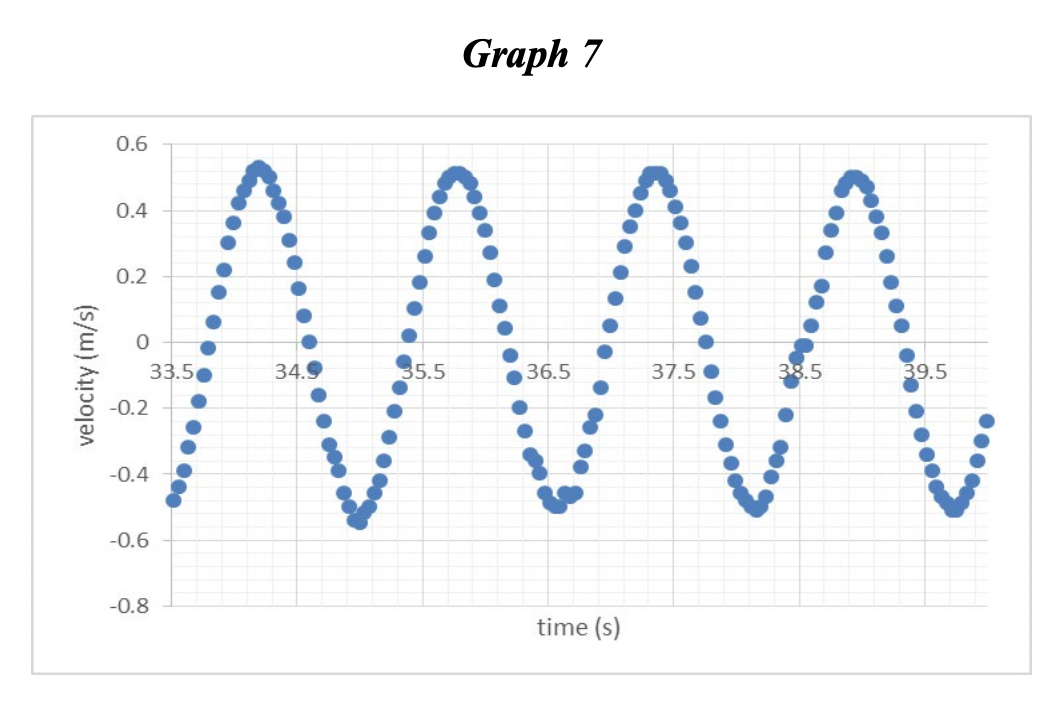
\includegraphics[width=\linewidth]{graph_7.png}
  \end{figure}

  \subsubsection{Graph Analysis}
  Graph 7 depicts some sort of oscillating motion. Because the graph is 
  sinusoidal, we know that the graph's position and acceleration will look
  just like the velocity, just shifted by some amount. This means that the 
  position is osciallting, as is the velocity and the acceleration.
  \subsubsection{Setup}
  In order to achieve the oscillating motion displayed, we decided to attach
  a weight to a spring. If we stretched the spring by some amount, then
  let go as we started recording the velocity, we knew that we could capture
  the same motion described by the graph.




  % \centerline{\textbf{Graph 1}}\\
  % % Any kind of straight lines, calculate a slope. D
  % \textbf{Graph 2}\\
  % \textbf{Graph 3}\\
  % \textbf{Graph 4}\\
  % \textbf{Graph 5}\\
  % \textbf{Graph 6}\\
  % \textbf{Graph 7}\\

  % \centerline{}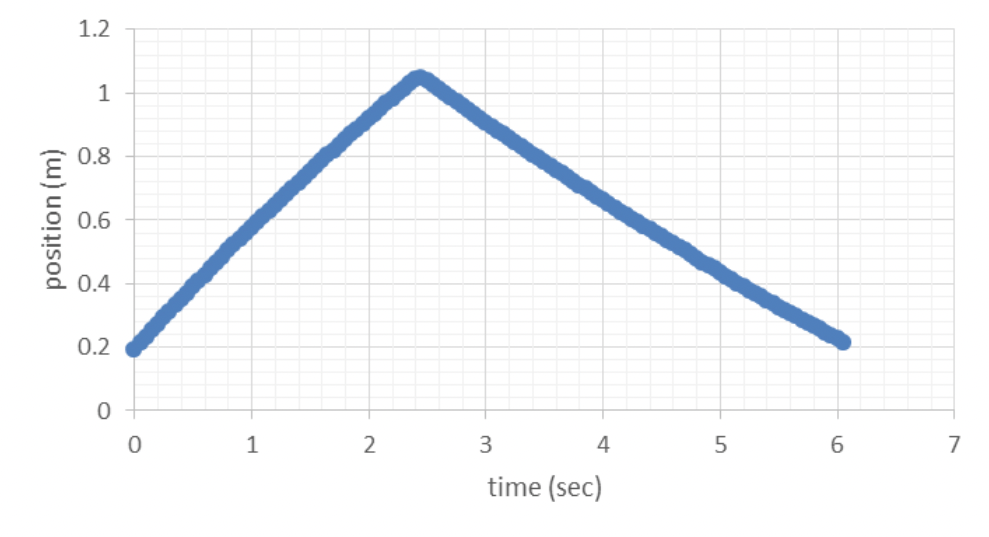
\includegraphics{graph_1.png}}

\end{document}

